%versi 2 (8-10-2016)
\chapter{Dasar Teori}
\label{chap:teori}

Dalam menjaga privasi data, perlu adanya definisi privasi yang konkrit untuk menentukan data seperti apa yang menjadi privasi. Pada penambangan data, perlu ada teknik yang baik untuk menjaga privasi tidak tersebar kepada orang yang tidak berhak. Ada beberapa teknik untuk menjaga privasi pada penambangan data antara lain modifikasi data dengan metode randomisasi yaitu teknik \textit{Random Rotation Perturbation} dan \textit{Random Projection Perturbation}

\section{Privasi Data}
\label{sec:privasidata} 

Pada umumnya sebuah data dapat dikatakan privasi apabila data tersebut dapat dikaitkan dengan identitas seseorang. Tetapi setiap orang memiliki kepentingan privasi yang berbeda-beda sehingga definisi dari privasi sulit untuk dijelaskan secara eksak. Oleh karena itu, perlu adanya konsep privasi yang dapat menjadi acuan untuk menentukan data seperti apa yang termasuk privasi atau bukan.

\subsection{Privasi}
\label{subsec:privasi}

Dalam mendefinisikan privasi, sulit untuk mendapatkan definisi yang tepat untuk privasi karena setiap individu memiliki kepentingan yang berbeda-beda sehingga privasi pada setiap individu dapat berbeda-beda juga. Beberapa definisi privasi telah dikemukakan dan definisi tersebut bermacam-macam berdasarkan konteks, budaya, dan lingkungan~\cite{stanleyosmar:04:standardppdm}. Menurut Warren dan Brandeis pada papernya, mereka mendefinisikan privasi sebagai “\textit{the right to be alone.}”, hak untuk menyendiri. Lalu pada papernya, Westin mendefinisikan privasi sebagai “\textit{the desire of people to choose freely under what circumstances and to what extent they will expose themselves, their attitude, and their behavior to others}”, keinginan orang untuk memilih secara bebas dalam segala situasi dan dalam hal mengemukakan diri mereka, sikap mereka, dan tingkah laku mereka pada orang lain. 

Schoeman mendefinisikan privasi sebagai “\textit{the right to determine what (personal) information is communicated to others}”, hak untuk menentukan informasi pribadi apa saja yang dikomunikasikan kepada yang lain, atau “\textit{the control an individual has over information about himself or herself.}”, kendali seorang individu terhadap informasi tentang dirinya sendiri. Lalu baru-baru ini, Garfinkel menyatakan bahwa “\textit{privacy is about self-possession, autonomy, and integrity.}”, privasi adalah tentang penguasaan diri sendiri, otonomi, dan integritas. Di samping itu, Rosenberg berpendapat bahwa privasi sebenarnya bukan sebuah hak tetapi sebuah rasa: “\textit{If privacy is in the end a matter of individual taste, then seeking a moral foundation for it -- beyond its role in making social institutions possible that we happen to prize -- will be no more fruitful than seeking a moral foundation for the taste for truffles.}”, intinya setiap orang memiliki perhatian yang berbeda-beda terhadap privasi mereka sendiri sehingga hal tersebut tergantung apa yang dirasakan oleh setiap individu.

Dari definisi-definisi privasi yang telah disebutkan di atas, dapat disimpulkan bahwa privasi dilihat sebagai konsep sosial dan budaya~\cite{stanleyosmar:04:standardppdm}. Konsep privasi pada suatu lingkungan dapat berbeda dari lingkungan lainnya dan hal ini menyebabkan sulitnya menentukan apakah sebuah data termasuk privasi atau bukan. Oleh karena itu, perlu adanya sebuah standar privasi untuk menentukan data mana yang dapat disebut sebuah privasi. Organisasi National Institute of Standards and Technology dari Amerika Serikat, membuat standar mereka sendiri untuk menentukan informasi seperti apa yang dapat disebut sebagai privasi. Mereka mengemukakan konsep \textit{Personally Identifiable Information} sebagai informasi yang dapat dikatakan personal untuk setiap individu.

\subsection{\textit{Personally Identifiable Information}}
\label{subsec:pii}

Privasi dapat dikatakan adalah sebuah informasi personal seseorang yang dapat mengidentifikasi suatu hal pada orang tersebut. Konsep yang sering kali digunakan untuk mendeskripsikan informasi personal adalah \textit{Personally Identifiable Information} yang disingkat PII. PII adalah segala informasi mengenai individu yang dikelola oleh sebuah instansi, termasuk segala informasi yang dapat digunakan untuk membedakan atau mengusut identitas seseorang dan juga segala informasi yang berhubungan atau dapat dihubungkan kepada suatu individu, seperti informasi medis, pendidikan, finansial, dan pekerjaan seseorang~\cite{nist:08:pii}. 

Informasi yang termasuk membedakan individu adalah informasi yang dapat mengidentifikasi seorang individu. Informasi seperti ini adalah data privasi yang secara langsung bisa didapatkan. Beberapa contoh informasi yang mengidentifikasi seorang individu adalah nama, nomor KTP, tempat tanggal lahir, nama ibu kandung, atau catatan medis. Sedangkan, data yang hanya berisi misalkan saldo tabungan tanpa ada informasi lain mengenai identitas seseorang yang berkaitan tidak menyediakan informasi yang cukup untuk mengidentifikasi seorang individu.

Dari sebuah data, bisa saja data tersebut secara tidak langsung mengandung privasi, identitas seseorang bisa didapatkan tanpa data tersebut memberikan langsung identitas orang tersebut. Mengusut identitas seseorang adalah proses dari membuat perkiraan tentang aspek spesifik dari aktivitas atau status seseorang. Jika sebuah data dapat dianalisis datanya sampai identitas seseorang dapat diakses, berarti data tersebut secara tidak langsung mengandung privasi. Contohnya adalah sebuah catatan finansial seseorang dapat digunakan untuk memperkirakan aktivitas dari individu tersebut.

Informasi yang berhubungan dapat didefinisikan sebagai informasi yang berkaitan dengan seorang individu yang mana terkait secara logis dengan informasi lain tentang individu tersebut. Informasi tersebut secara tidak langsung mengandung privasi dan dapat diolah agar identitas seseorang bisa didapatkan. Contohnya adalah apabila ada dua buah basis data yang memiliki data berbeda dari seorang individu, maka seseorang yang memiliki akses pada 2 basis data tersebut berpotensi dapat mengaitkan data-data tersebut lalu mengidentifikasi individu yang ada pada data tersebut.

\section{Penambangan Data}
\label{sec:penambangandata}

Pada era teknologi informasi, sangat banyak data terkumpul pada basis data. Data yang masif ini dapat dimanfaatkan untuk menggali informasi penting yang berguna untuk pembuatan keputusan. Proses pada aktivitas ini secara kasar dapat disebut dengan penambangan data.

Penambangan data adalah proses mengekstrak sebuah pola atau sebuah pengetahuan dari kumpulan data yang besar, yang mana dapat direpresentasikan dan diinterpretasikan~\cite{mendes:17:ppdmieee}. Pada penambangan data, teknik \textit{machine learning} dan \textit{pattern recognition} intensif digunakan untuk mendapatkan pola maupun pengetahuan baru dari data. Tujuan utama dari penambangan data adalah untuk membentuk model deskriptif dan prediktif dari suatu data. Model deskriptif berusaha untuk mengubah pola-pola yang ada pada data menjadi deskripsi yang dapat dimengerti oleh orang awam. Sedangkan model prediktif digunakan untuk memprediksi data yang tidak diketahui atau data yang berpotensi muncul di kemudian hari.

Model tersebut biasanya dibuat dengan menggunakan teknik \textit{machine learning}, yang mana terdapat dua teknik \textit{machine learning} yang paling sering digunakan yaitu \textit{classification} dan \textit{clustering}. Subbab berikutnya akan menjelaskan secara singkat kedua teknik tersebut dan contoh algoritmanya.

\subsection{\textit{Classification}}
\label{subsec:classification}

Tujuan utama \textit{Classification} (klasifikasi) adalah membuat model yang dalam kasus ini disebut \textit{classifier} yang mana dapat mengidentifikasi nilai kelas dari suatu data~\cite{mendes:17:ppdmieee}. Dalam kata lain, sebuah \textit{classifier} dibuat dari sebuah \textit{training set} dan model ini digunakan untuk mengklasifikasi data tidak diketahui ke dalam salah satu kelas.

Ada dua tahap dalam proses klasifikasi yaitu tahap latihan dan tahap klasifikasi. Pada tahap latihan, model akan dibuat dengan menggunakan \textit{training set}. \textit{Training set} yang dimaksud adalah data yang sudah diketahui kelasnya sehingga model yang ada melatih dirinya. Setelah \textit{classifier} terbentuk, barulah tahap klasifikasi dapat dilakukan dengan menggunakan \textit{classifier} yang tadi sudah dibuat. \textit{Classifier} akan memprediksi data yang kelasnya tidak diketahui. \textit{Classifier} akan semakin baik performanya seiring dengan banyaknya tahap latihan yang dilakukan.

Teknik \textit{machine learning} yang paling dikenal untuk klasifikasi antara lain \textit{K-nearest Neighbors}, \textit{Decision Tree}, dan \textit{Naive Bayes}. Dalam penelitian ini, hanya teknik \textit{K-nearest Neighbors} yang digunakan untuk pengujian sehingga berikutnya hanya akan dijelaskan teknik \textit{K-nearest Neighbors} saja. Teknik \textit{K-nearest Neighbors} adalah teknik penambangan data klasifikasi yang mencari label terbanyak pada sejumlah tetangga terdekatnya. Teknik ini bergantung pada jarak Euclidean antara titik yang merepresentasikan sebuah objek data yang akan diprediksi dengan titik-titik lain yang terdekat (tetangga-tetangganya). Setiap objek data pada dataset dipetakan ke bidang Euclidean dengan nilai dari beberapa atribut yang menentukan letaknya pada bidang Euclidean~\cite{jiawei:12:datmin}.

Berikut langkah kerja dari teknik \textit{K-nearest Neighbors}.
\begin{enumerate}
	\item Tentukan nilai \(k\) yang menentukan seberapa banyak tetangga yang digunakan
	\item Lakukan perulangan dengan iterasi sebanyak rekord yang ada selain rekord yang ingin diprediksi labelnya
	\begin{enumerate}
		\item Hitung jarak Euclidean antara rekord iterasi sekarang dengan rekord yang ingin diprediksi labelnya
		\item Catat jarak Euclidean dari rekord yang ingin diprediksi dan indeks rekord iterasi sekarang
	\end{enumerate}
	\item Urutkan jarak Euclidean titik-titik yang sudah dihitung pada perulangan pada langkah sebelumnya secara menaik
	\item Pilih rekord teratas (jarak Euclidean yang paling kecil) sebanyak \(k\) dari urutan pada langkah sebelumnya
	\item Ambil label dari semua rekord yang terpilih pada langkah sebelumnya. Label terbanyak adalah hasil prediksi label pada rekord yang ingin diprediksi
\end{enumerate}

Dalam mengevaluasi model klasifikasi dapat dihitung akurasi model dalam memprediksi suata data. Akurasi pada model klasifikasi berupa persentase jumlah prediksi yang benar dengan jumlah data yang diprediksi~\cite{jiawei:12:datmin}. Misalkan apabila model klasifikasi menebak dengan benar 8 buah objek data dari total berjumlah 10 objek data, berarti model tersebut memiliki akurasi sebesar 80\%.

\subsection{\textit{Clustering}}
\label{subsec:clustering}

\textit{Clustering} adalah proses mengelompokan kumpulan objek ke dalam sebuah kelompok (\textit{cluster}) sedemikian rupa sehingga objek-objek dari suatu \textit{cluster} memiliki lebih banyak kemiripan dari pada objek-objek dari \textit{cluster} lainnya~\cite{mendes:17:ppdmieee}. 

Salah satu contoh teknik \textit{clustering} adalah \textit{K-means}. Teknik \textit{k-means} adalah adalah teknik penambangan data \textit{clustering} yang memanfaatkan jarak Euclidean antara titik-titik yang ada untuk menentukan titik mana saja yang masuk ke kluster mana.

Berikut langkah kerja dari teknik \textit{K-means}.~\cite{jiawei:12:datmin}
\begin{enumerate}
	\item Tentukan nilai variabel \(k\) yang menentukan seberapa banyak kluster yang diinginkan dan sebuah \textit{treshold} untuk menentukan batas perubahan nilai \textit{centroid}
	\item Tentukan secara acak sebuah \textit{centroid} sebanyak \(k\)  untuk setiap kluster
	\item Lakukan perulangan sampai nilai fitur-fitur semua \textit{centroid} (titik tengah kluster) relatif tidak berubah atau dengan kata lain perubahannya kurang dari \textit{treshold}
	\begin{enumerate}
		\item Menghitung jarak Euclidean tiap titik dari \textit{centroid} ke titik tersebut dengan menggunakan beberapa fitur yang dipilih
		\item Kluster yang memiliki jarak Euclidean paling kecil dengan sebuah titik adalah kluster titik tersebut
		\item Tentukan kembali \textit{centroid} setiap kluster dengan cara menghitung rata-rata tiap fitur pada seluruh objek data pada kluster tersebut
	\end{enumerate}
\end{enumerate}

Dalam menentukan nilai variabel \textit{k} (jumlah \textit{cluster}) terbaik ada 2 metode yang dapat dipakai yaitu menghitung nilai \textit{Silhoutte Score} tertinggi dan metode Elbow. Metode Elbow bekerja dengan menggunakan  \textit{Sum of Squared Error} untuk membuat sebuah grafik hubungan antara nilai variabel \textit{k} dengan nilai \textit{Sum of Squared Error}. Penentuan nilai variabel \textit{k} dapat dilihat pada grafik tersebut nilai variabel \textit{k} mana yang perbedaan nilai \textit{Sum of Squared Error}-nya dengan nilai variabel \textit{k} sebelumnya memiliki perbedaan yang paling besar atau apabila dilihat pada grafiknya akan berbentuk seperti siku atau bengkokan.

\textit{Sum of Squared Error} adalah jumlah dari kuadrat jarak Euclidean setiap objek data terhadap \textit{centroid} pada masing-masing \textit{clusternya}~\cite{jiawei:12:datmin}. Rumus untuk menghitung \textit{Sum of Squared Error} dapat dilihat pada Persamaan~\ref{eq:sse}.
\begin{equation}\label{eq:sse}
	E = \sum^{k}_{i=1} \sum^{}_{p \in C_{i}} dist(\boldsymbol{p,c_{i}})^2
\end{equation}
Variabel \(\boldsymbol{p}\) adalah titik pada bidang Euclidean yang merepresentasikan sebuah objek data. Variabel \(\boldsymbol{c_{i}}\) adalah \textit{centroid} pada \textit{cluster} \(\boldsymbol{C_{i}}\).

\textit{Silhoutte Score} adalah rata-rata dari koefisien \textit{Silhoutte} setiap objek data yang ada. Sementara koefisien \textit{Silhoutte} adalah ukuran seberapa mirip suatu objek data dengan \textit{cluster}-nya sendiri dibandingkan dengan \textit{cluster} lain. Nilai dari koefisien \textit{Silhoutte} berada di antara -1 dan 1. Rumus untuk menghitung koefisien \textit{Silhoutte} dapat dilihat pada Persamaan~\ref{eq:silhoutte}.~\cite{jiawei:12:datmin}
\begin{equation}\label{eq:silhoutte}
	s(\mathbf{o}) = \frac{b(\mathbf{o})-a(\mathbf{o})}{\max{\{a(\mathbf{o}),b(\mathbf{o})}\}}
\end{equation}
Variabel \(\mathbf{o}\) adalah sebuah objek data. Fungsi \(a(\mathbf{o})\) adalah rata-rata jarak Euclidean antara sebuah objek data dan seluruh objek data pada \textit{cluster}-nya sendiri. Rumus dari fungsi ini dapat dilihat pada Persamaan~\ref{eq:ao}.
\begin{equation}\label{eq:ao}
	a(\mathbf{o}) = \frac{\sum^{}_{\mathbf{o'} \in C_{i},\mathbf{o}\neq\mathbf{o'}}dist(\mathbf{o},\mathbf{o'})}{|C_{i}|-1}
\end{equation}
Sementara fungsi \(b(\mathbf{o})\) adalah rata-rata jarak Euclidean paling kecil antara sebuah objek data dan seluruh objek data pada \textit{cluster} lain yang bukan \textit{cluster}-nya sendiri. Rumus dari fungsi ini dapat dilihat pada Persamaan~\ref{eq:bo}.
\begin{equation}\label{eq:bo}
	b(\mathbf{o}) = \min_{C_{j}:1\leq j \leq k,j\neq i}\left\{\frac{\sum^{}_{\mathbf{o'} \in C_{j}}dist(\mathbf{o},\mathbf{o'})}{|C_{j}|}\right\}
\end{equation}

\section{\textit{Privacy Preserving Data Mining}}
\label{sec:ppdm}

Aktivitas penambangan data melibatkan jumlah data yang sangat masif. Data-data yang digunakan memiliki privasi banyak individu di dalamnya. Hal ini berpotensi menyebabkan pelanggaran privasi dalam kasus tidak adanya proteksi yang cukup dan penyalahgunaan privasi data untuk tujuan lain~\cite{rezaseifi:11:ppdm}. Faktor utama pelanggaran privasi pada penambangan data adalah penyalahgunaan data sehingga hal ini dapat merugikan seorang individu maupun sebuah organisasi. Oleh karena itu, ada kebutuhan untuk menghindari penyebaran informasi pribadi yang rahasia maupun pengetahuan lainnya yang dapat diambil dari data yang digunakan untuk aktivitas penambangan data.

Konsep privasi sering kali lebih kompleks dari pada yang dibayangkan. Dalam kasus penambangan data, definisi dari menjaga privasi masih tidak jelas. Ada sebuah paper yang mendefinisikan \textit{privacy preserving data mining} sebagai “getting valid data mining results without learning the underlying data values”, mendapatkan hasil penambangan data yang valid tanpa  nilai pada data. Tetapi pada saat ini setiap teknik \textit{privacy preserving data mining} yang ada memiliki definisi privasinya masing-masing. 

Salah satu cara untuk melakukan \textit{privacy preserving data mining} adalah dengan melakukan modifikasi data yang ada sebelum diberikan kepada pihak lain. Berbagai macam pendekatan modifikasi data untuk \textit{privacy preserving data mining} telah dikembangkan antara lain \textit{Perturbation Approach} dan \textit{Anonymization Approach}, selengkapnya dapat dilihat pada Gambar~\ref{fig:ppdm}~\cite{rezaseifi:11:ppdm}. \textit{Perturbation Approach} adalah pendekatan untuk \textit{privacy preserving data mining} dengan cara mengacaukan data yang ada, tetapi hasil data yang dikacaukan masih tetap dapat ditambang. Sedangkan pada \textit{Anonymization Approach}, data diterapkan de-identifikasi di mana dataset mentah disebarluaskan setelah menghapus inti dari identitas setiap rekord~\cite{rezaseifi:11:ppdm}.

\textit{Perturbation Approach} dapat dibagi menjadi dua jenis lagi yaitu \textit{Value-based Perturbation Techniques} dan \textit{Multi-Dimensional Perturbation}. \textit{Value-based Perturbation Techniques} adalah teknik yang bekerja dengan cara menyisipkan \textit{random noise} pada data. Sedangkan terdapat dua jenis teknik \textit{Multi-Dimensional Perturbation} yaitu \textit{Data mining Task-based Perturbation} dan \textit{Dimension Reduction-based Perturbation}. \textit{Data mining Task-based Perturbation} adalah teknik yang bekerja dengan cara modifikasi data sehingga properti yang bertahan pada data yang telah dimodifikasi spesifik hanya properti yang digunakan oleh suatu teknik penambangan data tertentu. Sedangkan \textit{Dimension Reduction-based Perturbation} adalah teknik yang bekerja dengan cara modifikasi data sekaligus mengurangi dimensi dari data asli.

Hal yang sering kali diperhatikan pada teknik-teknik \textit{Perturbation Approach} adalah perbandingan antara jumlah privasi yang hilang dan jumlah informasi yang hilang. Idealnya teknik \textit{Perturbation Approach} yang baik adalah teknik yang fokus meminimalkan jumlah privasi yang hilang dan jumlah informasi yang hilang sehingga hasil penambangan dan akurasinya sama baiknya dengan tanpa menerapkan teknik \textit{Perturbation Approach}. Setiap teknik penambangan data memakai properti yang berbeda-beda pada data yang ditambang. Oleh karena itu, properti yang terjaga juga sebaiknya berdasarkan properti yang digunakan pada teknik penambangan data yang digunakan~\cite{rotation:05:chenliu}. Pada saat ini, teknik modifikasi data yang ada sering kali memiliki perbedaan pada properti-properti yang terjaga. Teknik-teknik modifikasi data tertentu sering kali memiliki fungsi yang berbeda atau teknik penambangan data yang dapat digunakan berbeda karena properti yang terjaga pada teknik-teknik tersebut berbeda juga.

\section{Metode \textit{Randomization}}
\label{sec:metoderandomization}

Dari berbagai macam teknik modifikasi data untuk \textit{privacy preserving data mining} yang dapat dilihat pada Gambar~\ref{fig:ppdm}, terdapat empat teknik yang menggunakan metode \textit{Randomization} yaitu \textit{Random Noise Addition}, \textit{Randomized Response}, \textit{Random Rotation Perturbation}, dan \textit{Random Projection Perturbation}.

Berbagai macam teknik dengan metode randomisasi umumnya menerapkan perusakan nilai pada data. Salah satu teknik yang pertama kali menggunakan metode randomisasi untuk \textit{privacy preserving data mining} adalah teknik \textit{Random Noise Addition} yang dikemukakan oleh Agrawal dan Srikant pada paper berikut~\cite{agrawalsrikant:00:randomnoise}. Teknik \textit{Random Noise Addition} ini dilakukan dengan cara menambahkan nilai random (\textit{noise}) pada data. Nilai random tersebut diambil dari sebuah distribusi. Untuk menambang data yang telah ditambahkan \textit{noise} ini perlu dilakukan rekonstruksi distribusi untuk mendapatkan distribusi yang asli. Oleh karena itu, teknik \textit{Random Noise Addition} ini hanya menjaga distribusi data asli sehingga hanya teknik penambangan data yang bergantung pada distribusi data saja yang dapat digunakan. Penyesuaian pada algoritma penambangan data yang digunakan juga perlu dilakukan agar teknik \textit{Random Noise Addition} ini dapat digunakan dan mendapatkan hasil penambangan data yang hampir sama dengan penambangan data tanpa menggunakan teknik \textit{Random Noise Addition}.

Setelah teknik \textit{Random Noise Addition} ditemukan, berbagai macam teknik lain juga dikembangkan terinspirasi dari teknik \textit{Random Noise Addition} ini. Teknik \textit{Random Rotation Perturbation} dan \textit{Random Projection Perturbation} adalah teknik adalah salah satunya, tetapi teknik tersebut tidak dilakukan dengan cara menambahkan \textit{noise} melainkan mengkalikan data asli dengan nilai random. Bagaimanapun juga, inti dari teknik-teknik randomisasi yang telah disebutkan di atas masih sama yaitu merusak data sehingga data yang dirilis bukanlah data asli melainkan data yang sudah rusak sehingga data yang dirilis tidak mengandung privasi sehingga privasinya terjaga. Masing-masing dari dua teknik tersebut akan dijelaskan lebih detil pada subbab-subbab berikutnya.

\subsection{\textit{Random Noise Addition}}
\label{subsec:rna}

Ide utama dari teknik \textit{Random Noise Addition}~\cite{agrawalsrikant:00:randomnoise} adalah mendistorsi nilai pada data dengan cara menambahkan \textit{random noise} yang diambil dari distribusi \textit{Uniform} atau \textit{Gaussian} dan memiliki rata-rata bernilai 0. Tetapi menurut penelitian yang telah dilakukan, distribusi \textit{Gaussian} lebih baik digunakan untuk teknik ini. \textit{Random noise} yang digunakan memiliki nilai yang berbeda untuk setiap nilai pada data.

Dengan teknik \textit{Random Noise Addition}, dari data yang sudah didistorsi bisa didapatkan kembali distribusi data asli dengan merekonstruksi distribusinya tanpa mendapatkan setiap nilai-nilai yang ada pada data asli. Metode rekonstruksi yang digunakan berdasarkan pada aturan \textit{Bayes}. Algoritma rekonstruksi untuk mendapatkan distribusi dari data asli dapat dilihat pada Gambar~\ref{fig:rnaalgorithm}.

\begin{figure}
	\centering
	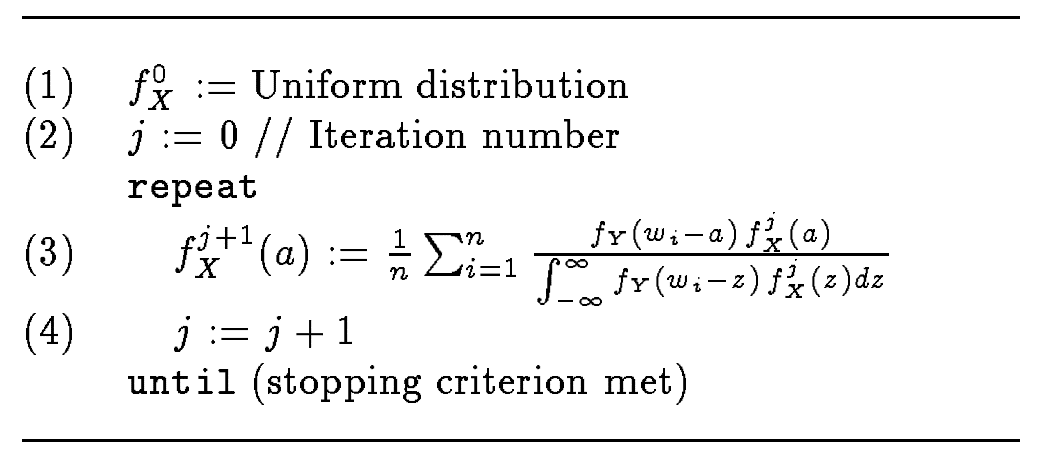
\includegraphics[scale=0.4]{rnaalgorithm}
	\caption{Algoritma rekonstruksi}
	\label{fig:rnaalgorithm}
\end{figure}

Algoritma ini berhenti sampai kriteria berhentinya terpenuhi. Kriteria tersebut adalah perbedaan estimasi distribusi iterasi sekarang dengan yang sebelumnya sangat kecil. Algoritma ini akan menghasilkan estimasi distribusi data asli dengan menggunakan data yang telah terdistorsi tanpa menggunakan nilai-nilai pada data asli, sehingga nilai-nilai pada data asli tidak tersebar. Oleh karena teknik \textit{Random Noise Addition} hanya menjaga distribusi pada data maka teknik penambangan data yang dapat digunakan hanya teknik-teknik yang bergantung pada distribusi data saja.

Modifikasi pada algoritma penambangan data yang digunakan juga perlu dilakukan. Contohnya apabila algoritma pohon keputusan digunakan, maka perlu modifikasi pada algoritma pohon keputusan tersebut. Hal ini menimbulkan masalah pada aplikasi pada dunia nyata karena tidak efisien dan memakan waktu untuk memodifikasi setiap algoritma yang ingin digunakan untuk menyesuaikan dengan teknik \textit{Random Noise Addition}. Masalah mengenai algoritma yang dapat digunakan juga menjadi perhatian karena teknik \textit{Random Noise Addition} hanya dapat digunakan untuk algoritma yang bergantung pada distribusi saja sedangkan teknik randomisasi lain tidak menjaga distribusi pada data. Ada juga penelitian yang mengatakan bahwa teknik \textit{Random Noise Addition} ini memiliki kualitas yang kurang baik dalam menjaga privasi data karena banyaknya celah yang dapat diserang pada teknik ini. Oleh karena masalah-masalah tersebut, akhirnya teknik ini juga tidak akan digunakan untuk penelitian ini. Teknik \textit{Random Projection Perturbation} akan digunakan untuk menggantikan teknik \textit{Random Noise Addition}.

\subsection{\textit{Random Rotation Perturbation}}
\label{subsec:rrp}

Ide utama dari teknik \textit{Random Rotation Perturbation} adalah jika data direpresentasikan sebagai matriks \(X_{n \times d}\) , \textit{rotation perturbation} dari dataset X didefinisikan sebagai berikut.
\begin{equation}
	G(X) = X_{n \times d} R_{d \times d}
\end{equation}
Dimana \(R_{d \times d}\) adalah \textit{random rotation matrix}. \textit{Random rotation matrix} berukuran \(d\) dimensi dapat dibuat dengan cara membuat matriks \textit{special orthogonal} acak karena matriks rotasi memiliki sifat {special orthogonal}. Matriks \textit{special orthogonal} adalah matriks yang memiliki sifat \textit{orthogonal} dan determinannya bernilai +1, yang mana matriks \textit{orthogonal} adalah matriks yang menghasilkan matriks identitas apabila dikalikan dengan transposenya sendiri. Matriks rotasi ini dapat dibuat secara efisien mengikuti distribusi Haar~\cite{stewart:80:orthogonal}. Dari definisi di atas dapat disimpulkan tranformasi rotasi tersebut menjaga jarak Euclidean~\cite{rotation:05:chenliu}.

Teknik ini menjaga beberapa properti pada data antara lain yaitu jarak Euclidean, \textit{inner product}, dan \textit{geometric shape hyper} pada bidang multi-dimensi~\cite{rezaseifi:11:ppdm}. Oleh karena itu, beberapa teknik penambangan data tidak berpengaruh (dapat digunakan) terhadap teknik \textit{Random Rotation Perturbation} antara lain yaitu \textit{K-nearest Neighbors}, \textit{Support Vector Machines}, dan \textit{Perceptrons}~\cite{rotation:05:chenliu}. Teknik ini dipercaya dapat memberikan hasil penambangan yang maksimal, hasil penambangan data yang telah dirusak persis sama dengan hasil penambangan data aslinya. Sehingga jumlah informasi yang hilang tidak ada, tetapi jumlah privasi yang hilangnya tinggi. Walaupun demikian ada beberapa penelitian yang mengatakan bahwa karena teknik \textit{Random Rotation Perturbation} ini memiliki sifat demikian sehigga teknik ini dikatakan tidak aman dan dapat diserang dengan beberapa teknik untuk mendapatkan data asli yang lengkap.

Transformasi translasi juga perlu dilakukan agar rotasi yang dilakukan merusak data secara menyeluruh. Apabila tidak dilakukan translasi, nilai pada data yang mendekati nilai nol akan menghasilkan nilai yang mendekati nol juga setelah dirotasi. Implikasi dari hal tersebut adalah lemahnya dalam menjaga privasi. Translasi dapat dilakukan dengan cara membuat matriks translasi yang acak lalu kalikan dengan matriks data asli. Translasi dapat dilakukan karena translasi tidak mengubah properti geometris dari matriks yang ditranslasi sehingga jarak Euclidean terjaga dan hasil penambangan data yang bergantung pada jarak Euclidean tetap sama.

\subsubsection{Algoritma}
\label{subsubsec:algo-rotation}

Algoritma \textit{Random Rotation Perturbation} memiliki beberapa langkah yaitu sebagai berikut.
\begin{enumerate}
    \item Dataset yang memiliki atribut sebanyak \(d\) dan rekord sebanyak \(n\) direpresentasikan dalam bentuk matriks berukuran \(n \times d\)
    \item Buatlah matriks translasi acak yang diambil mengikuti distribusi \textit{uniform} dengan rentang [0, 100] berdimensi \((d+1)\times(d+1)\)
    \item Untuk keperluan transformasi translasi, matriks dataset perlu ditambahkan sebuah kolom dengan nilai 1 pada seluruh barisnya.
    \item Lakukan transformasi translasi dengan cara mengkalikan matriks dataset dengan matriks translasi yang telah dibuat pada langkah kedua
    \item Oleh karena keperluan transformasi translasi, hasil translasi akan berupa matriks berdimensi \(n\times(d+1)\) dengan kolom terakhir berisi nilai 1 pada setiap barisnya. Oleh karena itu, kolom tersebut perlu dibuang agar dimensi matriks dataset kembali sesuai aslinya \(n \times d\)
    \item Buatlah \textit{random rotation matrix} berukuran \(d \times d\) dengan membuat matriks \textit{orthogonal} acak. Matriks \textit{orthogonal} memiliki sifat yaitu determinannya sebesar 1 dan hasil perkalian matriks tersebut dengan transposenya adalah matriks identitas
    \item Lakukan transformasi rotasi dengan cara mengkalikan matriks dataset dengan \textit{random rotation matrix} yang telah dibuat pada langkah keenam
    \item Hasil matriks yang telah dirotasi sudah dapat langsung digunakan untuk penambangan data
\end{enumerate}

\subsection{\textit{Random Projection Perturbation}}
\label{subsec:rpp}

Ide utama dari teknik \textit{Random Projection Perturbation} adalah mereduksi dimensi dari representasi matriks data asli dengan syarat dimensi matriks tersebut cukup besar. Dasar dari teknik \textit{Random Projection Perturbation} berdiri pada \textit{Johnson-Lindenstrauss Lemma}.~\cite{lindestrauss:84:jllemma}
\newtheorem{theorem}{Lemma}
\begin{theorem}[\textit{JOHNSON-LINDENSTRAUSS LEMMA}]
	For any \(0 < \epsilon < 1\) and any integer \(s\), let \(k\) be a positive integer such that \(k\) \(\geq 4(\epsilon^{2}/2-\epsilon^{3}/3)^{-1}\ln{n}\). Then, for any set \(S\) of \(s = |S|\) data points in \({\rm I\!R}^{m}\), there is a map \(f : {\rm I\!R}^{m} \rightarrow {\rm I\!R}^{k}\) such that, for all \(x, y \in S\), \((1-eps)||u - v||^{2}<||p(u) - p(v)||^{2}<(1+eps)||u - v||^{2}\), where \(||.||\) denotes the vector 2-norm.
\end{theorem}
Inti dari Lemma ini menunjukkan bahwa titik pada bidang Euclidean \(d\)-dimensi dapat diproyeksikan ke bidang Euclidean berdimensi lebih kecil dari \(d\) tetapi jarak Euclidean antara dua titik tetap terjaga dengan distorsi yang terkontrol tetapi dengan syarat \(d\) harus cukup besar. Oleh karena adanya distorsi yang muncul, akurasi pada model yang dibuat dengan data tersebut akan berkurang dibandingkan data aslinya.~\cite{kargupta:06:projection}

\textit{Projection perturbation} dari dataset X didefinisikan sebagai berikut.
\begin{equation}
	G(X) = X_{n \times d} R_{d \times k}
\end{equation}
Dimana \(R_{d \times k}\) adalah \textit{random projection matrix} yang dihasilkan mengikuti distribusi normal, dengan rata-rata bernilai 0 dan standar deviasi bernilai \(1/\sqrt{k}\). Ukuran matriks \(R_{d \times k}\) disesuaikan dengan matriks \(X_{n \times d}\) yang mana dataset asli dengan jumlah rekord \(n\) dan jumlah atribut \(d\), yang mana \(d\) adalah jumlah fitur pada dataset atau dimensi matriks tersebut. Tentunya dalam mereduksi dimensi nilai \(k\) harus lebih kecil dari pada \(d\), yang mana \(k\) adalah dimensi dari matriks baru yang dihasilkan dari \textit{Random Projection Perturbation} ini.

Jika \textit{random projection matrix} yang digunakan dihasilkan secara acak saja, hasil dari \textit{random projection perturbation} akan terlalu merusak nilai pada data sehingga akurasi pada model yang akan dibuat kemungkinan berkurang drastis. Cara menanggulangi hal tersebut adalah menggunakan matriks \textit{orthogonal} sebagai \textit{random projection matrix}. Tetapi membuat matriks \textit{orthogonal} yang berdimensi tinggi memiliki kompleksitas yang tinggi sehingga memerlukan \textit{cost} yang besar. Pada observasi yang dilakukan Hecht-Neilsen menunjukkan bahwa “\textit{that in a high-dimensional space, vectors with random directions are almost orthogonal}”~\cite{bingham:01:projection}. Dapat disimpulkan bahwa dalam kasus matriks berdimensi tinggi apabila sebuah matriks dihasilkan secara acak mengikuti suatu distribusi, matriks tersebut akan kurang lebih hampir \textit{orthogonal}. Oleh karena itu, matriks yang dibuat untuk \textit{Random Projection Perturbation} cukup matriks acak yang mengikuti suatu distribusi saja.

Menurut \textit{Johnson-Lindenstrauss Lemma}, reduksi dimensi pada matriks berdimensi tinggi minimal berdimensi \(k\), yang mana \(k\) didefinisikan sebagai berikut.
\begin{equation}
	k \geq 4(\epsilon^{2}/2-\epsilon^{3}/3)^{-1}\ln{n}
\end{equation}
Sebuah matriks yang akan diproyeksikan ke dimensi yang lebih kecil akan memiliki distorsi pada jarak Euclidean yang dimiliki oleh titik-titik (setiap elemen dari matriks) pada bidang Euclidean tersebut. Distorsi tersebut ditentukan oleh variabel \(\epsilon\), yang mana \(\epsilon\) menjadi ukuran seberapa baik proyeksi dilakukan. Semakin kecil nilai \(\epsilon\) maka semakin besar \(k\), yang mana \(k\) adalah dimensi minimal matriks yang dihasilkan. Semakin titik-titik pada bidang Euclidean diproyeksikan ke dimensi lebih kecil, semakin besar kerusakan yang timbul pada jarak Euclidean titik-titik tersebut.

Persamaan berikut menyatakan rentang error yang terjadi pada \textit{Random Projection Perturbation} dengan \(\epsilon\) (eps) yang ditentukan berada pada rentang (0, 1). 
\begin{equation}
	(1-eps)||u - v||^{2}<||p(u) - p(v)||^{2}<(1+eps)||u - v||^{2}
\end{equation}
Pada hasil proyeksi, jarak Euclidean antara suatu titik dengan suatu titik lainnya dapat dipastikan berada pada rentang tersebut dan tidak akan melebihi distorsi yang ditentukan.

\subsubsection{Algoritma}
\label{subsubsec:algo-projection}

Algoritma \textit{Random Projection Perturbation} memiliki beberapa langkah yaitu sebagai berikut.
\begin{enumerate}
    \item Dataset yang memiliki atribut sebanyak \(d\) dan rekord sebanyak \(n\) direpresentasikan dalam bentuk matriks berukuran \(n \times d\)
    \item Tentukan nilai variabel \(\epsilon\) (epsilon) yang diinginkan dan berada pada rentang (0, 1)
    \item Hitung nilai minimal variabel \(k\) (dimensi minimal) dengan rumus berikut \(k \geq 4(\epsilon^{2}/2-\epsilon^{3}/3)^{-1}\ln{n}\)
    \item Tentukan nilai variabel \(k\) yang diinginkan dengan memenuhi persyaratan pada langkah ketiga dan nilai variabel \(k\) yang dipiilih harus lebih kecil dari \(d\) (dimensi dataset aslinya)
    \item Buatlah matriks proyeksi berukuran \(d \times k\) dengan cara membuat matriks acak yang diambil mengikuti distribusi normal dengan rata-rata bernilai 0 dan standar deviasi bernilai \(1/\sqrt{k}\)
    \item Lakukan proyeksi dengan cara mengkalikan matriks dataset dengan matriks proyeksi yang telah dibuat pada langkah kelima
    \item Hasil matriks yang telah diproyeksi sudah dapat langsung digunakan untuk penambangan data
\end{enumerate}

\section{Bahasa Pemograman Python Beserta \textit{Library}-nya}
\label{sec:metoderandomization}

Bahasa pemograman Python~\cite{python:95:guido} adalah bahasa pemograman yang sudah umum digunakan untuk melakukan penambangan data. Oleh karena itu, komunitas pada bahasa pemograman Python sudah sangat besar dan banyak pihak yang membuat \textit{library} dan \textit{tools} yang mendukung dalam melakukan penambangan data pada bahasa pemograman ini. Tetapi bahasa pemograman Python tidak semata-mata hanya dapat digunakan untuk penambangan data, Python merupakan bahasa pemograman yang multifungsi dan banyak juga digunakan pada bidang lain selain penambangan data. Bahasa pemograman Python dapat juga digunakan untuk membuat antarmuka dengan dukungan \textit{framework} tertentu. Selain itu, Python juga merupakan bahasa pemograman yang berorientasi objek. Berikut akan dijelaskan beberapa \textit{library}, \textit{framework}, dan \textit{tools} yang berguna untuk membuat antarmuka perangkat lunak, mendukung implementasi metode \textit{Randomization}, dan mendukung proses penambangan data.

\begin{itemize}
	\item Kivy\footnote{https://kivy.org/} adalah \textit{framework} yang berfungsi untuk membuat antarmuka perangkat lunak. Kivy dapat membuat antarmuka perangkat lunak pada berbagai \textit{platform} seperti Windows, OS X, Android, iOS, dan Raspberry Pi.
	\item Numpy dan Scipy~\cite{2020SciPy-NMeth} adalah \textit{library} yang berfungsi untuk memanipulasi struktur data matriks atau melakukan operasi matematis yang berkaitan struktur data \textit{array} atau matriks. Contohnya yang dipakai pada penelitian ini adalah membuat matriks \textit{orthogonal} secara acak.
	\item Pandas~\cite{mckinney-proc-scipy-2010} adalah \textit{library} yang berfungsi untuk menganalisis dan memanipulasi data berbentuk struktur data yang lebih kompleks seperti \textit{dataframe}. Pandas juga menyediakan fungsi untuk membaca dokumen dan mengkonversinya ke struktur data \textit{dataframe} dan sebaliknya.
	\item Scikit-learn~\cite{scikit-learn} adalah \textit{library} yang berfungsi untuk melakukan proses pembelajaran mesin dan memiliki berbagai macam fungsi pembelajaran mesin yang dapat digunakan untuk penambangan data seperti teknik \textit{k-nearest neighbors} dan \textit{k-means}.
	\item Matplotlib~\cite{Hunter:2007}, Plotly\footnote{https://plotly.com/}, dan Seaborn\footnote{https://seaborn.pydata.org/} adalah \textit{library} yang berfungsi untuk melakukan berbagai macam visualisasi dengan mudah. Contohnya yang dipakai pada penelitian ini adalah visualisasi dengan \textit{scatter plot} dan \textit{line plot}.
	\item Spyder\footnote{https://www.spyder-ide.org/} adalah sebuah perangkat lunak \textit{integrated development environment} (IDE) yang berfungsi sebagai editor dan \textit{compiler} bahasa pemograman Python serta berfungsi untuk menampilkan berbagai macam visualisasi. Perangkat lunak ini sudah umum digunakan untuk penambangan data karena kemudahannya.
	\item Anaconda\footnote{https://www.anaconda.com/} adalah \textit{tools} yang berfungsi sebagai \textit{platform data science} dengan bahasa pemograman Python yang memudahkan pengguna dalam manajemen \textit{package}, \textit{setup} seluruh perangkat lunak, \textit{library}, IDE, dan berbagai macam keperluan lainnya yang berkaitan dengan bahasa pemograman Python serta berbagai hal yang mendukung proses penambangan data.
\end{itemize}